%Thanks for Rapport CentraleSupelec - Template, By Axel Poupart-Lafarge

\documentclass{rapportCS}
\usepackage{lipsum}
\usepackage{algorithm2e}
\usepackage{subcaption}
\title{Global Illumination Study: Achieving Indirect Lighting}
\RestyleAlgo{ruled}


\begin{document}


\titre{Global Illumination Study: Achieving Indirect Lighting}
\pieddepage{GI Study: Achieving Indirect Lighting}


\mention{Game Programming} % Nom de la formation
\master{GPU Specialization} % Nom de l'option choisie
\trigrammemention{MGP2 - GPU} % Pour le bas de la page


\eleve{Rémi GINER, Jarod SENGKEO, Rayane TADJER}

\dates{11/10/2024 - 04/06/2025}

% Informations tuteurs ISART
\tuteuruniv{
    \textsc{Maël ADDOUM} \\ m.addoum@isartdigital.com
    \textsc{Aurélien LHERBIER} \\ a.lherbier@isartdigital.com
    \textsc{Maxime ROUFFET} \\ maximerouffet@gmail.com
} 

        
\fairemarges %Afficher les marges

\fairepagedegarde %Créer la page de garde


\section*{Abstract}
\addcontentsline{toc}{section}{\protect\numberline{}Abstract}

Write abstract here.


\newpage



\contents % Créer la table de matières



\newpage

\section{Introduction} 

This paper explores different Global Illumination (GI) algorithms through a GPU-specialized project at Isart DIGITAL Paris. We implemented various GI algorithms and compared them. The implementations include a classical GI algorithm with Image-Based Irradiance Probes and a new approach called Radiance Cascades. These two algorithms are implemented in a custom, rendering engine built with Vulkan.

Global illumination, also known as Indirect Lighting, enables photorealistic visuals by accurately simulating how light interacts within a scene. Several techniques simulate indirect lighting; most of the classical implementations of GI use irradiance probes. These probes gather their irradiance and apply it to the surrounding objects.
    
Among the innovative approaches in this domain, the Radiance Cascades algorithm has emerged as a significant contribution to real-time GI techniques. Originally introduced and refined by researchers and practitioners such as Alexander Sannikov, Jason Today, and Alexander Griffis, Radiance Cascades leverages cascaded data structures to efficiently approximate light propagation. We focus on two GI techniques: Radiance Cascades and Image-Based Lighting with Irradiance Probes. Radiance Cascades is an alternative to these latter. It is a new algorithm implemented in the game Path of Exile 2. Its adoption in a AAA title underscores its viability for real-time rendering, particularly in environments requiring high-quality indirect lighting. While most implementations to date remain confined to 2D scenarios, this paper also explores the emerging potential of its 3D variants by assessing their feasibility and performance in modern rendering systems.

Through this project, we build on the work of previous contributors and extend the body of knowledge surrounding Global Illumination. By experimenting with various algorithms, we design a hypothetically ultimate algorithm candidate. Additionally, we reduce the gap between experimental research and real-world application in Global Illumination by providing the main points of interest surrounding this rendering technique to new contributors.


\section{State of the Art}

details of each existing techniques


\section{Methodology}
The goal of this paper was to compare two different approaches to know how to achieve Global Illumination; we chose to study two different Indirect Lighting algorithms: the first one being completely new and experimental and the second one being classic and naive.


\subsection{Work environment}
In order to have an accurate comparison, we implemented our custom rendering engine instead of just analyzing existing code. This choice was made to prevent any other unexpected results or a polluted environment.

The first task to do in this study was to create a suitable working environment. We created a Render Hardware Interface (RHI) to use the Vulkan API more easily. Our RHI allows us to create a Vulkan context and manage all the required objects (e.g. device, command buffers, memory, buffers, and images).

\begin{figure}
\centering
\rule{1cm}{1cm}
\caption{UML of our application architecture}
\end{figure}

\begin{figure}
\centering
\rule{1cm}{1cm}
\caption{UML of the rendering architecture used}
\end{figure}

Once the engine was ready to render in 3D, a 2D renderer was also implemented to prepare the implementation of the Radiance Cascades algorithm in 2D. However, a first proof-of-concept using the Shadertoy website.

Because the scope of this study is only to describe the implementation of indirect lighting, the final results do not have the vocation to be physically-based in any form.
Choosing to reimplement different approaches gives us the opportunity to learn and to spot the precise implications of each technique. By doing this we planned to learn a lot from these two techniques to make our own 3D implementation of Radiance Cascades.


\subsection{Radiance Cascades in 2D}
The first technique we started to recreate is Radiance Cascades, the technique described in Alexander Sannikov’s research paper for the game Path of Exile 2.

We first implemented the Radiance Cascades techniques in 2D to follow the thinking path of the original researcher Alexander Sannikov. Also, many programmers, who have implemented it, have first done it in 2D. It is a simpler way to think of the many rays. It is called Flatland.
The Radiance Cascades technique is composed of layers of probes arranged in a grid. Each probe will gather the radiance information using a “raycasting function” \cite{}.

Once the implementation is done on Shadertoy, it will be ported to our custom rendering engine. This is mandatory to achieve quality rendering and good performances because the implementation on WebGPU was quite naive. It uses encoding and decoding the probes position and radiance intervals using fragment shaders as well. This encoding technique is made at each frame, which causes several performance issues. It is the reason why we cannot increase the number of probes on this naive approach.

\begin{figure}
\centering
\rule{1cm}{1cm}
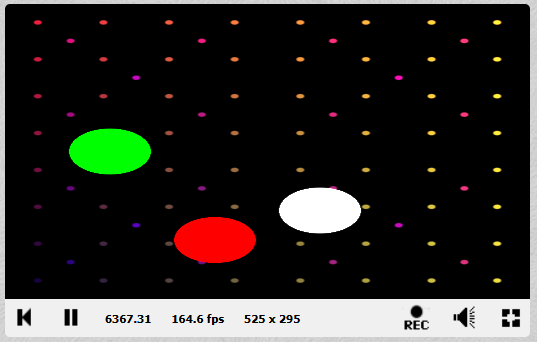
\includegraphics{figures/shadertoy/shadertoy_cascades.png}
\caption{Probes arranged in a cascade on Shadertoy}
\end{figure}

On the custom engine we will implement a CPU side custom probe management system. This will allow us to pass information to the GPU using buffers instead of recreating every data structure in the fragment shaders.


\subsection{Global Illumination with Irradiance Probes}
The second technique we started to recreate is Global Illumination with Irradiance Probes. This approach was chosen because of its probe usage, like Radiance Cascades and because of its simplicity and straightforwardness.
The current implementation we made is based on Irradiance Maps generated with scene capture made by probes placed in a grid. Because we are concerned only with diffuse lighting, the low precision of Irradiance Maps is tolerable. In the future, this implementation may change to use Spherical Harmonics instead of Irradiance Maps.
Dynamic Diffuse Global Illumination (DDGI) is not in the scope of this project, this technique discards the influence of probes that are not visible by a fragment (e.g., the probe is behind a wall). Omitting this technique helps to highlight the weaknesses of this algorithm.
Because we based our work on a Vulkan Engine, we were able to use techniques such as multiview rendering, which allows us to render a scene in a cubemap using one draw call, and removes a potential performance bottleneck.


\subsection{Radiance Cascades in 3D}
In order to have a proper comparison and similar performance the Radiance Cascades technique should be ported in a 3D environment. This brings trilinear interpolation from the previously described technique into the game.

\subsubsection{Raycasting function}
The raycasting function is implemented as follows:


\begin{algorithm}[hbt!]
\caption{Naive uniform raycasting function}\label{alg:two}
\KwResult{The color of the pixel from the raycast hit result}
$maxIterationCount \gets x$\;
$length \gets y$\;
$stepSize \gets \frac{length}{maxIterationCount}$\;
$sampledPoint \gets raycastOrigin$\;
\For{$i \gets 0$ to $maxIterationCount$}{
$sampledColor \gets colorFromWorld$\;
$sampledPoint \gets sampledStep + raycastDir * stepSize$\;
}
\end{algorithm}


But it should be implemented using a grid:


\begin{algorithm}[hbt!]
\caption{Raycasting function in a grid}\label{alg:two}
\KwResult{The color of the pixel from the raycast hit result}
$length \gets y$\;
$sampledPoint \gets raycastOrigin$\;
\For{$i \gets 0$ to $maxIterationCount$}{
$sampledColor \gets colorFromWorld$\;
$sampledPoint \gets sampledStep + variableLengthDependingOnTheGrid$\;
}
\end{algorithm}

\begin{figure}
\centering
\rule{1cm}{1cm}
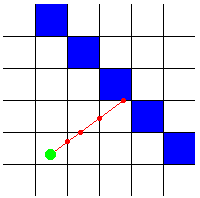
\includegraphics{figures/raycast_grid.png}
\caption{A grid for 2D raycasting as described in Lode Vandevenne’s blog post}
\end{figure}

This gives a rather scene-independent raycasting function because the sampling moves along a virtual grid rather than uniformly or with Signed-Distance Functions like in raymarching.
In 3D, multiple algorithms allow us to use raycasting to find a collision such as the collision algorithms. In order to keep the raycasting function technique scene independent, it then needs a 3D grid, a voxel grid.

We also theorized the usage of scene capture of 1 * 1 pixel to have a similar result to the raycasting function to avoid the implementation of a voxel grid but this technique should not remain scene independent as it should draw each object of the scene.

For the 3D Radiance Cascades implementation, another approach came into mind: Image-Based Radiance Cascades. Which works by mixing our naive approach of Global Illumination with Irradiance Probes and Radiance Cascades to get the best of the two worlds: being a straightforward implementation in 3D and being scaled for high-precision quite easily. Its memory and performance footprint still have to be tested. 
Like the 2D implementation of Radiance Cascades, this algorithm works firstly by placing layers of probes in multiple grids of different resolutions. Then, for each probe, a scene capture is made to generate a texture gathering the irradiance of the environment. The resolution of the texture depends on the cascade index of the probe. Because the first cascade is made of probes that cast 8 rays in 3D (4 rays in 2D), this behavior can be replicated by drawing the scene in a texture made of 8 layers of 1px. For the second cascade, the capture will result in a 32x1px because of the 32 raycasts needed in 3D.
This approach also helps to gather the depth of the environment easily. It also raises a lot of problems, such as losing the scene-independent property of the base algorithm and the appearance of possible bottlenecks with draw calls, which can be resolved using batching. The two other potential problems are the cost of overlapped triangles during the rendering process because of the low resolution of the framebuffer, and the fact that long-distance objects are captured by low-linear-resolution-probes if batching is used. These problems may be fixed using Level of Detail (LOD) or GPU-based frustum culling.
Finally, the resulting irradiance of each probe can be merged, as was the case in 2D.




\section{Results}

The results should include implementation specifics and profiling statistics. Indeed, the implemented algorithms are done with our work style, from our own comprehension of the diverse research papers.
The statistics are used to make visible the implications of each technique. It is also used to prove the least consuming algorithm with the better visual result.


\subsection{Implementation}
The first part of our study is to implement each technique before going to the second part, comparing. Therefore we have some implementation results.

\subsubsection{Radiances Cascades in 2D}

In 3D, the indirect lighting is the pixels lit by a light reflection (or a light bounce). This can be visualized with a Cornell Box, where a white object appears red because of the wall’s color. It is different in 2D. Because the objects are not visible with their surface but with their “interior”, the indirect lighting is represented as “volumetric light” in the 2D atmosphere.

\begin{figure}
\centering
\rule{1cm}{1cm}
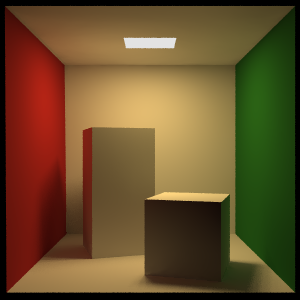
\includegraphics{figures/cornell_box.png}
\caption{Image of a Cornell Box from Wikipedia}
\end{figure}


\begin{figure}[!htb]
   \begin{minipage}{0.48\textwidth}
     \centering
     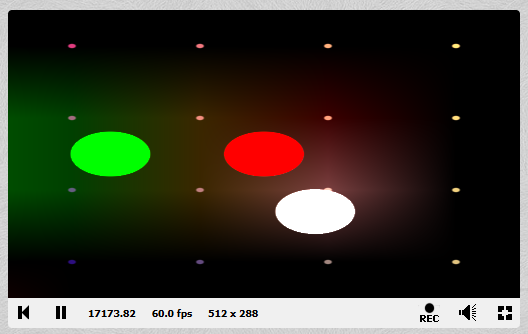
\includegraphics[width=.7\linewidth]{figures/shadertoy/shadertoy_no_shadows.png}
   \end{minipage}\hfill
   \begin{minipage}{0.48\textwidth}
     \centering
     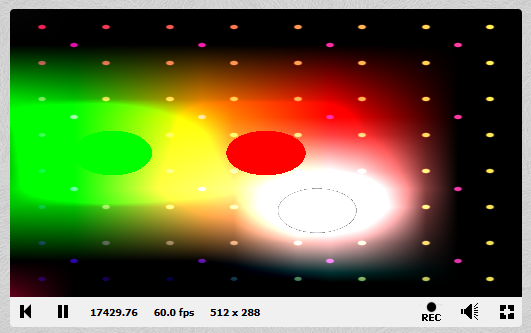
\includegraphics[width=.7\linewidth]{figures/shadertoy/shadertoy_no_shadows2.png}
   \end{minipage}
    \caption{First attempt of applying radiance to the “atmosphere” pixels}
\end{figure}

Some debug tools have also been implemented in the post process shader to visualize the areas of the atmosphere affected by the indirect light.

\begin{figure}
\centering
\rule{1cm}{1cm}
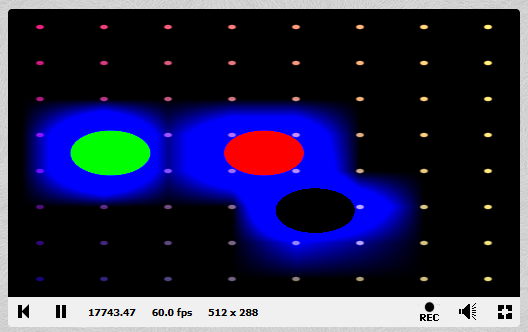
\includegraphics{figures/shadertoy/shadertoy_affection.png}
\caption{Debugging pixels affected by the probes}
\end{figure}

Bilinear interpolation is used to calculate the combination of probes interval into the computed pixels.



\begin{figure}[!htb]
   \begin{minipage}{0.48\textwidth}
     \centering
     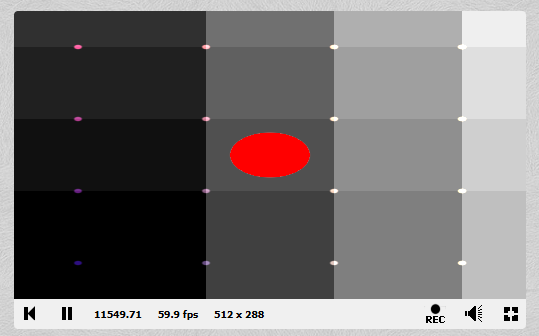
\includegraphics[width=.7\linewidth]{figures/shadertoy/shadertoy_bilerp.png}
   \end{minipage}\hfill
   \begin{minipage}{0.48\textwidth}
     \centering
     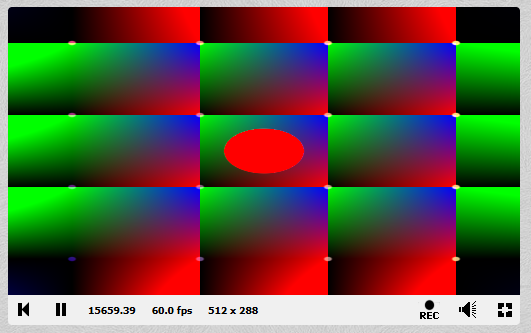
\includegraphics[width=.7\linewidth]{figures/shadertoy/shadertoy_bilerp_2.png}
   \end{minipage}
    \caption{Areas of the atmosphere affected by the probes using bilinear interpolation}
\end{figure}

The shadows and penumbra are visible in the final result but some problems still remain such as Light Leaks or poor visual quality.

\begin{figure}
\centering
\rule{1cm}{1cm}
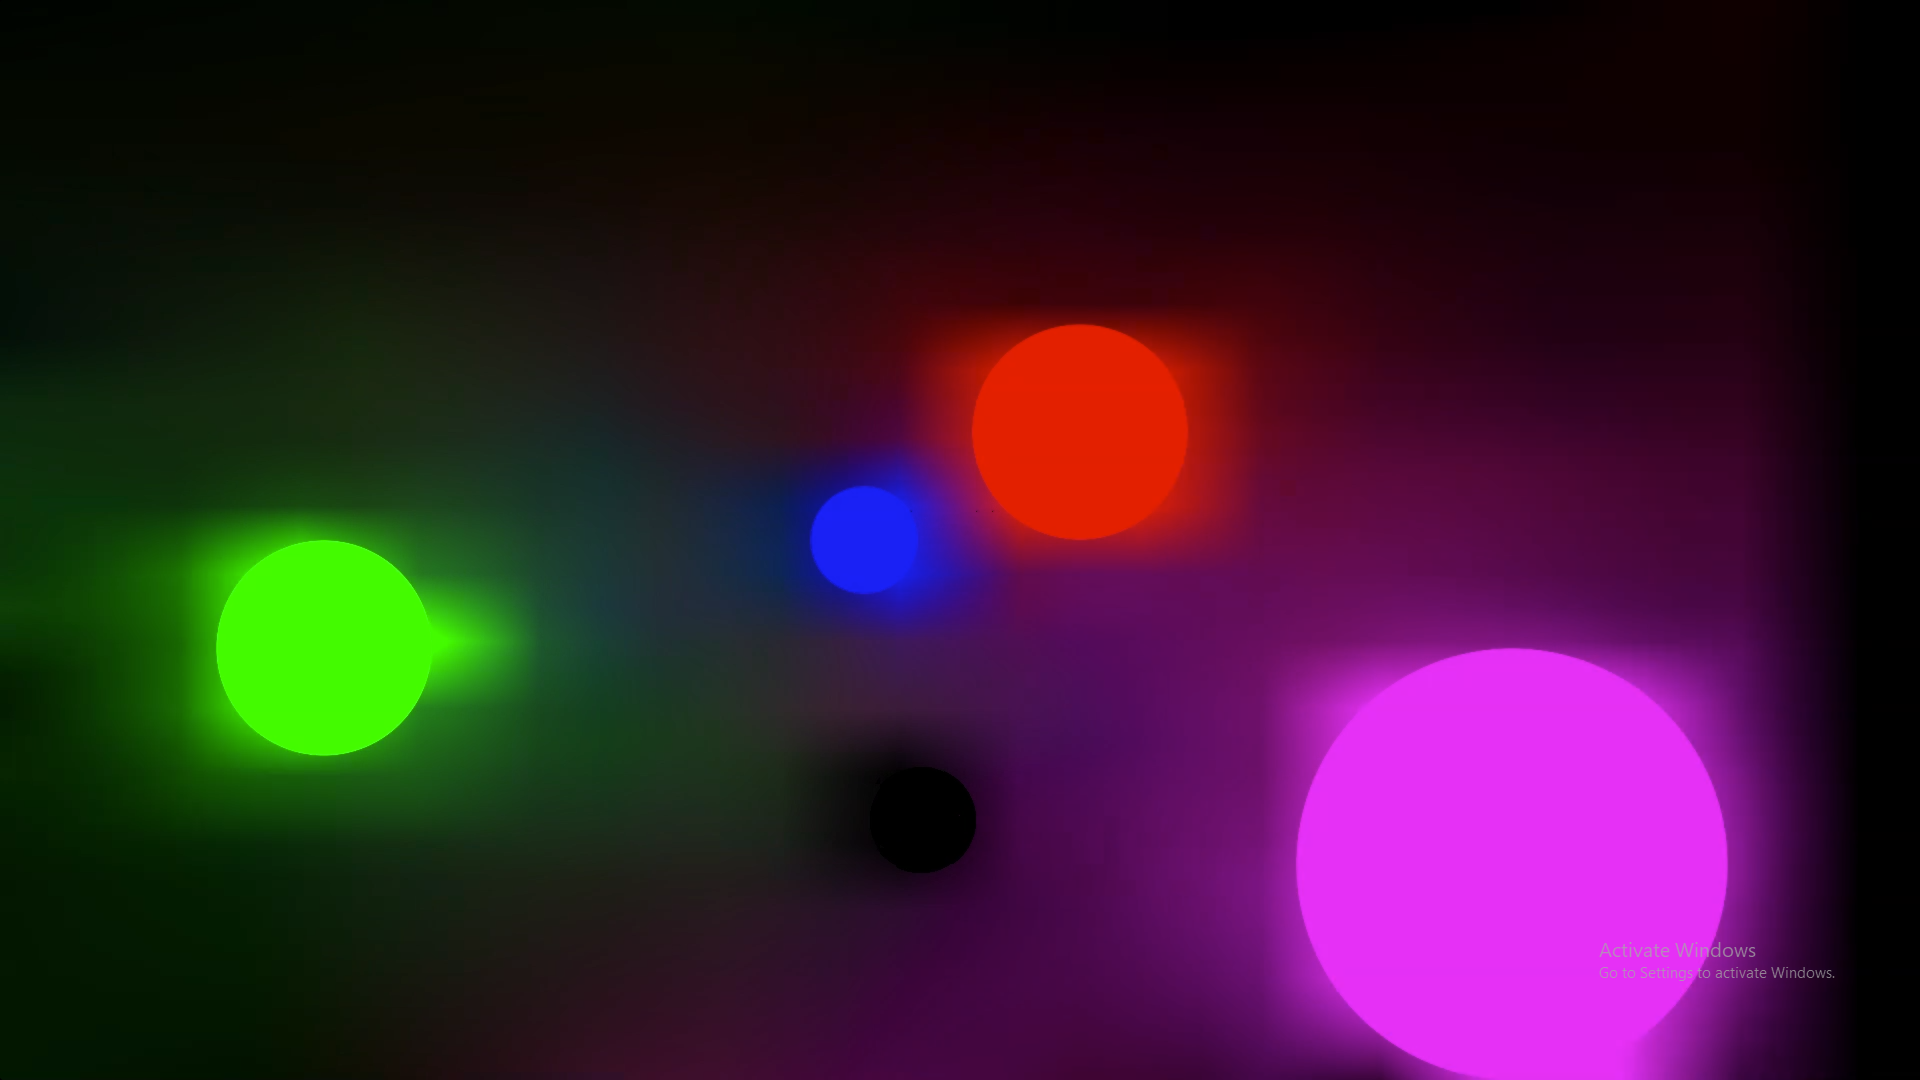
\includegraphics[width=1\linewidth]{figures/shadertoy/shadertoy_final_cubic.png}
\caption{Final result with visible shadows and penumbra with the pink light}
\end{figure}

\begin{figure}
\centering
\rule{1cm}{1cm}
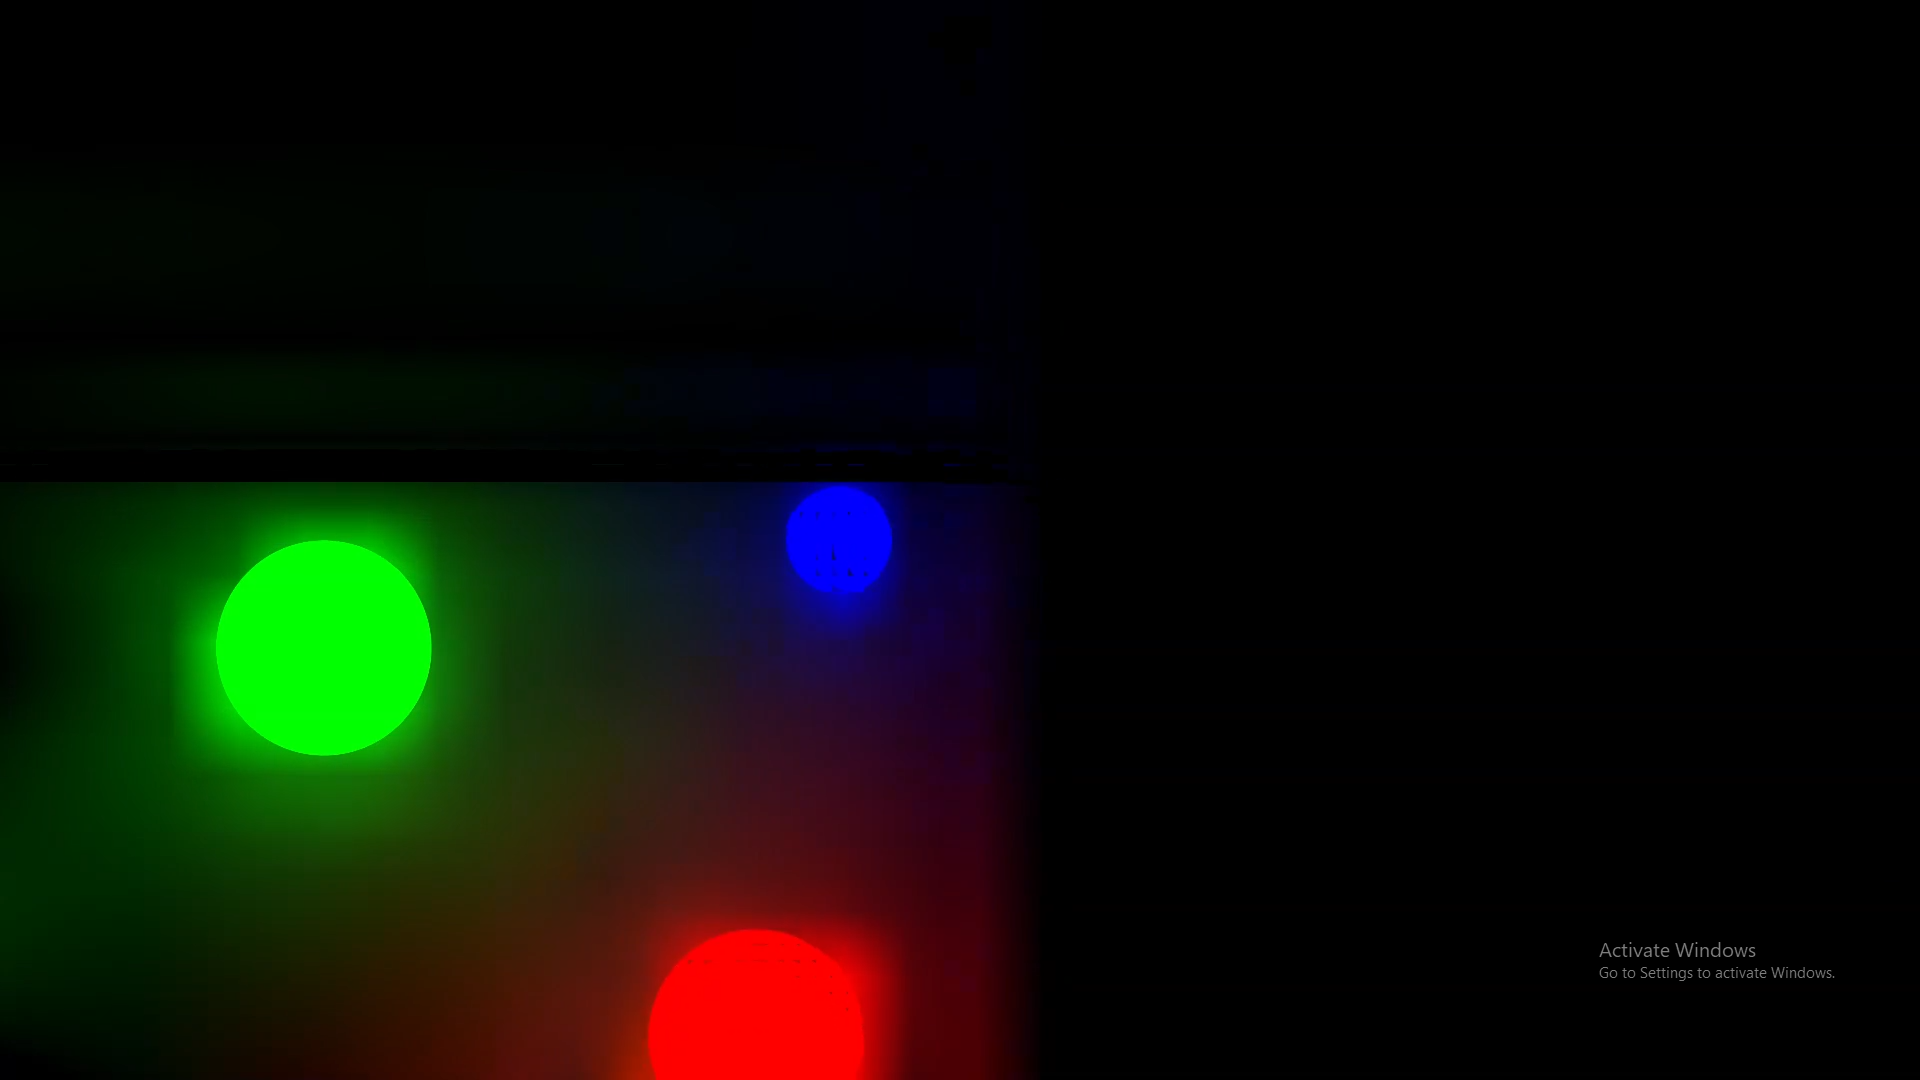
\includegraphics[width=1\linewidth]{figures/shadertoy/shadertoy_final_leaks.png}
\caption{Final result with light leaking visible for the green light}
\end{figure}

\subsubsection{Global Illumination with Irradiance Probes}
After implementing Radiance Cascades in Shadertoy and Global Illumination with Irradiance Probes using Irradiance Maps, our first results were here. 

\begin{figure}
    \begin{subfigure}{0.33\textwidth}
        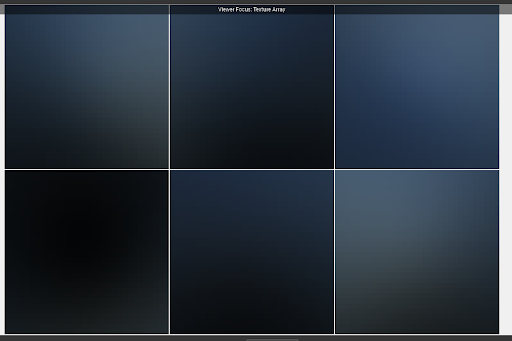
\includegraphics[width=1\linewidth]{figures/irradiance-map-1.png}
        \caption{Irradiance Maps generated with the skybox.}
        \label{fig:subim1}
    \end{subfigure}\hfill
    \begin{subfigure}{0.33\textwidth}
        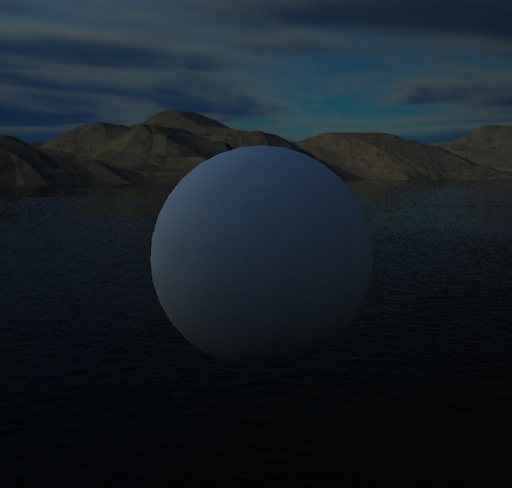
\includegraphics[width=1\linewidth]{figures/ibl-result-1.png}
        \caption{Debug sphere to display Irradiance Maps.}
        \label{fig:subim2}
    \end{subfigure}\hfill
    \begin{subfigure}{0.33\textwidth}
        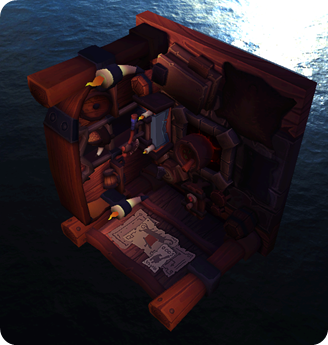
\includegraphics[width=1\linewidth]{figures/ibl-result-2.png}
        \caption{Scene lit by the skybox indirect lighting.}
        \label{fig:subim3}
    \end{subfigure}
    \caption{Indirect lighting from skybox.}
\end{figure}

\begin{figure}
    \begin{subfigure}{0.5\textwidth}
        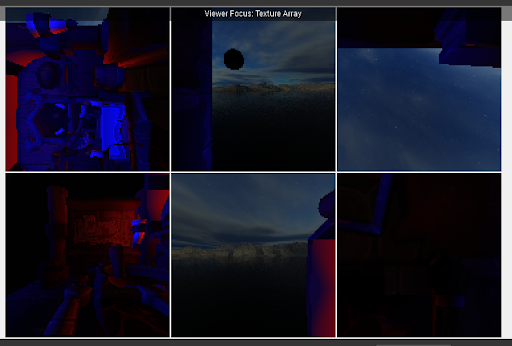
\includegraphics[width=1\linewidth]{figures/scene-capture.png}
        \caption{Scene captured by a probe in a cubemap.}
        \label{fig:subim4}
    \end{subfigure}\hfill
    \begin{subfigure}{0.5\textwidth}
        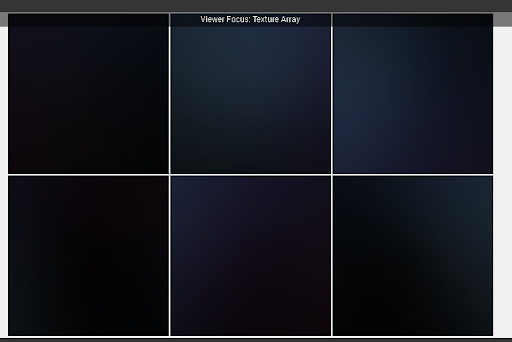
\includegraphics[width=1\linewidth]{figures/irradiance-map-2.png} 
        \caption{Irradiance Map associated with the scene capture.}
        \label{fig:subim5}
    \end{subfigure}
    \caption{Indirect lighting from scene shading and geometry.}
\end{figure}

\begin{figure}
    \begin{subfigure}{0.5\textwidth}
        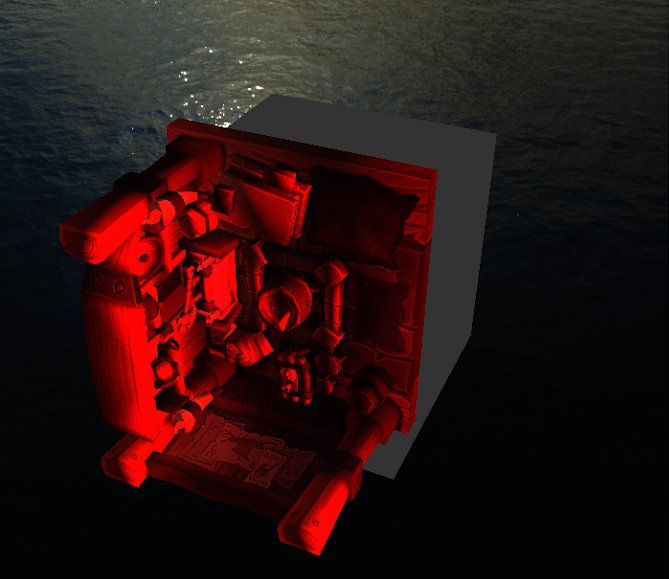
\includegraphics[width=1\linewidth]{figures/ibl-result-3.png}
        \caption{Scene lit in red with direct lighting.}
        \label{fig:subim6}
    \end{subfigure}\hfill
    \begin{subfigure}{0.5\textwidth}
        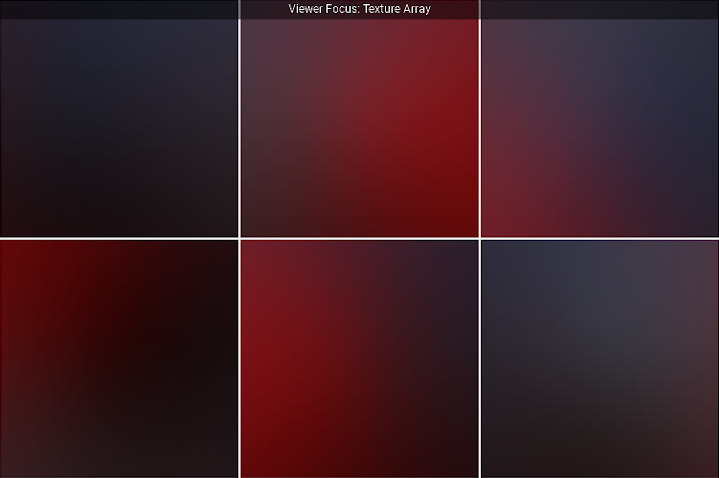
\includegraphics[width=1\linewidth]{figures/irradiance-map-3.png} 
        \caption{Irradiance Maps showing the influence of the direct lighting.}
        \label{fig:subim7}
    \end{subfigure}
    \caption{Influence of the direct lighting on indirect lighting.}
\end{figure}

\subsubsection{Radiance Cascades in 3D}

\subsection{Profiling}
Each technique has its implications in memory usage or in frame time.
The second studied technique was not convincing in terms of performance. 


\section{Observations}

\section{Conclusion}

\section*{Lexicon}
\addcontentsline{toc}{section}{\protect\numberline{}Lexicon}


\subsection*{Definitions}
\addcontentsline{toc}{subsection}{\protect\numberline{}Definitions}

Many expressions are used throughout this paper, the definitions are below. Those expressions correspond to the terms used in the industry.

Light source: Object directly emitting light (e.g. lamp, sun, fire, …).

Emission:

Direct Lighting: Lighting of a pixel using the angle towards the light source, such as in the Phong algorithm.

Luminance: Light emitted by a lit object or a light source (term used in physics).

Indirect Lighting: Lighting of a pixel using the surrounding lit objects.

Global Illumination: Algorithm used to calculate the final amount of light of a pixel, combining direct and indirect lighting.

Image-Based Lighting: Lighting of a pixel using an Irradiance Map.

Probe: Object, usually spherical, placed in the world to capture the surrounding lighting data in the position of the probe precisely (it can be used for radiance but for reflections as well).

Radiance: Similar to the luminance.

Irradiance: Final amount of light received at a certain point (such as a pixel in computer graphics)

Irradiance Map: Texture, usually a cubemap, used to encode a radiance field to be used as irradiance.

Cubemap: Six-faced texture.

Radiance Probe: Probe used to capture the surrounding radiance.

Irradiance Probe: Probe used to capture the surrounding radiance and let access to its data to apply the radiance on the nearby objects as irradiance.

Global Illumination with Irradiance Probes: Technique that uses irradiance probes to encode the radiance data and whether uses irradiance maps or spherical harmonics to describe the irradiance data.

Cascade: Data structure that contains layers of similar data. The layers may have different parameters (e.g. Radiance Cascades, Cascaded Shadow Mapping).

Radiance Cascades: Global Illumination technique created by Alexander Sannikov described in his paper.

Flatland: Term to describe a scene in 2D.

Cornell Box: Typical and rather simple scene to demonstrate lighting features.

Raycasting:

Raytracing:

Raymarching:

Signed-Distance Function:

Static: Non moving object. Non state-changing algorithm.

Baking: Precomputing a calculation to facilitate the real-time execution requiring its result.

Dynamic:

Ambient:

Diffuse: Part of an object directly lit by a light source.

Specular: Part of an object lit by a light source and that reflects the most amount of light into the viewer’s eye.

Reflection:

Light bounce: Light hitting its final destination after being reflected by a more or less reflective object.

Atmosphere: Area unoccupied by physical objects.

Volumetric Light: (or Volume Light) is a type of lighting where the participating media make the rays of light visible.

Shadow:

Penumbra:

Light Leak: (or Leaking)

Participating media: Small particles in the air that render the beam of light visible.

Render Hardware Interface: Wrapper that allows the user to utilize graphics API such as Vulkan or OpenGL.

Shadertoy: A website by Pol Jeremias and Iñigo Quilez that allows users to write fragment shaders using GLSL.

Shader: Program that runs on a Graphics Card using a Graphics API.

Fragment Shader: Part of a shader that is executed for every pixel of the rendered image.

Buffer: Data structure sent to the Graphics Card.

Interpolation:

Linear Interpolation:

Bilinear Interpolation:

Trilinear Interpolation:


\subsection*{Abbreviations}
\addcontentsline{toc}{subsection}{\protect\numberline{}Abbreviations}

GI: Global Illumination

IBL: Image-Based Lighting

DDGI: Dynamic Diffuse Global Illumination

LOD: Level of Detail

SDF: Signed-Distance Function

RHI: Render Hardware Interface

API: Application Programming Interface

UML: Unified Modeling Language

GLSL: OpenGL Shading Language

CPU: Central Processing Unit

GPU: Graphics Processing Unit

\section*{Personalities}
\addcontentsline{toc}{section}{\protect\numberline{}Personalities}

Rémi Giner - Student

Jarod Sengkeo - Student

Rayane Tadjer - Student

Maël Addoum - Supervisor, m.addoum@isartdigital.com

Aurélien LHERBIER - Supervisor, a.lherbier@isartdigital.com

Maxime ROUFFET - Supervisor, maximerouffet@gmail.com

Malek Bengougam - Graphics Engineer

Alexander Sannikov - Graphics Engineer

Lode Vandevenne - Graphics Engineer

Pol Jeremias - Creator of Shadertoy

Iñigo Quilez - Creator of Shadertoy




\section*{Bibliographical References}
\addcontentsline{toc}{section}{\protect\numberline{}Bibliographical References}


\bibliography{Bib/myBib} % This is required to be included
\bibliographystyle{unsrt} % vous pouvez utiliser d'autres styles pour lister vos références (regardez sur internet) 

\newpage


\end{document}
  